% Appendix F — supplementary figures

These supplementary figures back the two main-text figures (Fig.~\ref{fig:headline}, Fig.~\ref{fig:withinpr}) with more detail on distributional and cross-cell behaviour.

\begin{figure}[h]
    \centering
    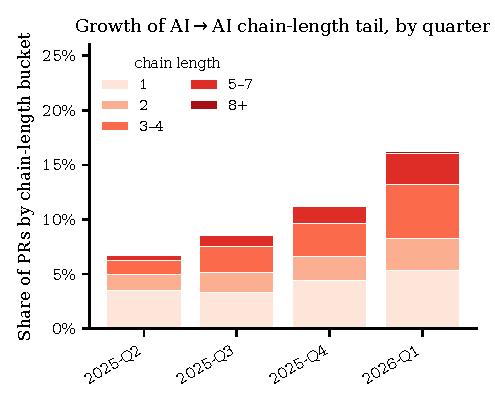
\includegraphics[width=0.55\linewidth]{figures/figure2_chain_length.pdf}
    \caption{Distribution of longest AI$\to$AI chain length per PR, by quarter. Boxes show the interquartile range with whiskers at 1.5$\times$IQR. Fliers are omitted. Annotations report the quarterly mean and $p_{95}$. The tail grows monotonically: $p_{95}$ triples from 2025-Q2 to 2026-Q1. The single-PR maximum (13) is stable, indicating growth driven by more \emph{PRs} having long chains rather than any one PR having an unprecedentedly long chain.}
    \label{fig:chainbox}
\end{figure}
